%Author, Company
\documentclass[11pt,a4paper,ngerman, fleqn]{article}

%Importierte Packete
\usepackage[a4paper,text={160mm,255mm}]{geometry}
\usepackage[utf8]{inputenc}
\usepackage[T1]{fontenc}
\usepackage{lmodern}
\usepackage{babel}
\usepackage{amsmath}
\usepackage[babel,german=quotes]{csquotes}
\usepackage{graphicx}
\usepackage{amssymb}
\usepackage{multirow}
\usepackage{textcomp}
\usepackage[margin=10pt,font=small,labelfont=bf]{caption}
\usepackage[stable]{footmisc}
\usepackage{tikz}
\usepackage[colorlinks=true,linkcolor=black, urlcolor=OPTIMAblue]{hyperref}
\usepackage{listings}
\usepackage{color}
\usepackage{float}
\usepackage{ragged2e}
\usepackage{pdflscape}
\usepackage{pdfpages} 
\usepackage{setspace}
\usepackage{mathtools}
\usepackage{pifont}
\usepackage[nohyperlinks]{acronym}

%Zeilenabstand
\onehalfspacing

%Definierte Farben
\definecolor{mygreen}{rgb}{0,0.6,0}
\definecolor{OPTIMAblue}{RGB}{0,140,194}
\definecolor{mygray}{rgb}{0.5,0.5,0.5}
\definecolor{mymauve}{rgb}{0.58,0,0.82}
\definecolor{slightgray}{RGB}{238,233,233}
\definecolor{pureblack}{RGB}{0,0,0}
\definecolor{purewhite}{RGB}{255,255,255}

%Definition der Farbe von Verweisen
\hypersetup{  colorlinks=true,
		  citecolor=pureblack} 

%Sourcecode Implementierung
\lstset{ %
  language=C,
  backgroundcolor=\color{slightgray},	% choose the background color; you must add \usepackage{color} or \usepackage{xcolor}
  basicstyle=\ttfamily\footnotesize,	% the size of the fonts that are used for the code
  breakatwhitespace=false,         		% sets if automatic breaks should only happen at whitespace
  breaklines=true,                 			% sets automatic line breaking
  captionpos=b,                    			% sets the caption-position to bottom
  commentstyle=\color{mygreen},   	% comment style
  deletekeywords={...},            			% if you want to delete keywords from the given language
  keywordstyle=\color{blue}, 
  morekeywords={FOR, TO, BY, DO, END_FOR, IF, END_IF, FUNCTION_BLOCK, TRUE, FALSE, THEN, CASE, OF, ADR, SIZEOF, REAL_TO_INT, SQRT, INT_TO_REAL, AND, OR, NOT, ABS, LOG, END_FUNCTION_BLOCK, END_CASE, FUNCTION, END_FUNCTION},
  escapeinside={\%*}{*)},          		% if you want to add LaTeX within your code
  extendedchars=true,              		% lets you use non-ASCII characters; for 8-bits encodings only, does not work with UTF-8
  frame=single,                    			% adds a frame around the code
  keepspaces=true,                			% keeps spaces in text, useful for keeping indentation of code
  numbers=left,                    			% where to put the line-numbers; possible values are (none, left, right)
  numbersep=5pt,                   			% how far the line-numbers are from the code
  numberstyle=\tiny\color{black}, 		% the style that is used for the line-numbers
  rulecolor=\color{black},         		% if not set, the frame-color may be changed on line-breaks within not-black text
  showspaces=false,                		% show spaces everywhere adding particular underscores; it overrides 'showstringspaces'
  showstringspaces=false,          		% underline spaces within strings only
  showtabs=false,                  			% show tabs within strings adding particular underscores
  stepnumber=1,                    			% the step between two line-numbers. If it's 1, each line will be numbered
  stringstyle=\color{mymauve},     		% string literal style
  tabsize=4,                       			% sets default tabsize to 2 spaces
}

%Shortcuts Umbenennungen
\let\qt\enquote
\let\noi\noindent
\let\tbf\textbf

%Befehle
\newcommand\circlearound[1]{%
  \tikz[baseline]\node[draw,shape=circle,anchor=base] {#1} ;}

\newcommand{\kreis}[1]{\unitlength1ex\begin{picture}(2.5,2.5)%
\put(0.75,0.75){\circle{2.5}}\put(0.75,0.75){\makebox(0,0){#1}}\end{picture}}

%Globale Dokumenteninformationen
\date{\today}
\author{Felix Binder}
\begin{huge}
\title{\textbf{Echtzeitsysteme - Übung} \vspace{10mm} \\ \LARGE C - Tutorial Zusammenfassung}
\end{huge}

%+++++++++++++++++++++++++++++++++++++++++++++++++++++++++++++++++++++++++++++
%				 Titelblatt + Inhaltsverzeichnis
%+++++++++++++++++++++++++++++++++++++++++++++++++++++++++++++++++++++++++++++
\begin{document}

\renewcommand{\theequation}{\arabic{section}.\arabic{equation}}
\maketitle

\thispagestyle{empty}

\newpage
\pagenumbering{Roman}
\setcounter{page}{1}

%Inhaltsverzeichnis
\tableofcontents

\newpage
\pagenumbering{arabic}
\setcounter{page}{1}
 
%+++++++++++++++++++++++++++++++++++++++++++++++++++++++++++++++++++++++++++++
%					     Vorwort
%+++++++++++++++++++++++++++++++++++++++++++++++++++++++++++++++++++++++++++++
\section*{Vorwort}
\addcontentsline{toc}{section}{Vorwort}

Alle hier verwendeten Beispiele stammen aus dem C-Tutorial von Elias Fischer \cite{1}. Dieses Dokument fasst das Tutorial lediglich auf seine elementaren Bestandteile zusammen.

\newpage

%++++++++++++++++++++++++++++++++++++++++++++++++++++++++++++++++++++++++++++
%					  1.1  Hello World
%++++++++++++++++++++++++++++++++++++++++++++++++++++++++++++++++++++++++++++
\section{Einführung}
\subsection{\qt{Hello World!}}
\label{sec:11}


Datei: \tbf{HelloWorld.c}

\begin{lstlisting}
#include<stdio.h>

int main() {
	printf("Hello World\n");
	return 0;
}
\end{lstlisting}

\noi Kompilieren der Hochsprache zu ausführbarem Maschinencode unter UNIX:

\begin{lstlisting}[language=bash,  backgroundcolor=\color{pureblack}, basicstyle=\ttfamily\footnotesize\color{purewhite}, rulecolor=\color{slightgray}]
  $ gcc -o HelloWorld HelloWorld.c
\end{lstlisting}

\noi Maschinencode ausführen mit Ergebnis im Terminal.

\begin{lstlisting}[language=bash,  backgroundcolor=\color{pureblack}, basicstyle=\ttfamily\footnotesize\color{purewhite}, rulecolor=\color{slightgray}]
  $ ./HelloWorld
  $ Hello World!
\end{lstlisting}

%++++++++++++++++++++++++++++++++++++++++++++++++++++++++++++++++++++++++++++
%					  1.2  Kommentare
%++++++++++++++++++++++++++++++++++++++++++++++++++++++++++++++++++++++++++++
\subsection{Kommentare}
\label{sec:12}


Datei: \tbf{HelloWorld.c}

\begin{lstlisting}
#include<stdio.h>

int main() {
	//printf("Diese Zeile ist auskommentiert!\n");
	
	/*
	printf("Diese Zeilen\n");
	printf("sind ebenfalls\n");
	printf("auskommentiert\n");
	*/
	
	printf("Ziemlich leer oder?\n");
	return 0;
}
\end{lstlisting}

\begin{lstlisting}[language=bash,  backgroundcolor=\color{pureblack}, basicstyle=\ttfamily\footnotesize\color{purewhite}, rulecolor=\color{slightgray}]
  $ ./HelloWorld
  $ Ziemlich leer oder?
\end{lstlisting}

%++++++++++++++++++++++++++++++++++++++++++++++++++++++++++++++++++++++++++++
%					  1.3  Hexadezimal
%++++++++++++++++++++++++++++++++++++++++++++++++++++++++++++++++++++++++++++

\subsection{Hexadezimale Zahlen}
\label{sec:13}


Datei: \tbf{HelloWorld.c}

\begin{lstlisting}
#include<stdio.h>

int main() {
	int tmp = 0xFF;
	printf("Zahl: %d\n", tmp);
	return 0;
}
\end{lstlisting}

\begin{lstlisting}[language=bash,  backgroundcolor=\color{pureblack}, basicstyle=\ttfamily\footnotesize\color{purewhite}, rulecolor=\color{slightgray}]
  $ ./HelloWorld
  $ Zahl: 255
\end{lstlisting}

\noi Schlüsselwort: \tbf{0x}..

%++++++++++++++++++++++++++++++++++++++++++++++++++++++++++++++++++++++++++++
%					  1.4  Binäre Zahlen
%++++++++++++++++++++++++++++++++++++++++++++++++++++++++++++++++++++++++++++

\subsection{Binäre Zahlen}
\label{sec:14}


Datei: \tbf{HelloWorld.c}

\begin{lstlisting}
#include<stdio.h>

int main() {
	int tmp = 0b0101;
	printf("Zahl: %d\n", tmp);
	return 0;
}
\end{lstlisting}

\begin{lstlisting}[language=bash,  backgroundcolor=\color{pureblack}, basicstyle=\ttfamily\footnotesize\color{purewhite}, rulecolor=\color{slightgray}]
  $ ./HelloWorld
  $ Zahl: 5
\end{lstlisting}

\noi Schlüsselwort: \tbf{0b}....

%++++++++++++++++++++++++++++++++++++++++++++++++++++++++++++++++++++++++++++
%					  2.1  Elementare Datentypen
%++++++++++++++++++++++++++++++++++++++++++++++++++++++++++++++++++++++++++++
\section{Variablen}
\subsection{Elementare Datentypen}
\label{sec:21}


\begin{figure}[H]
	\centering
	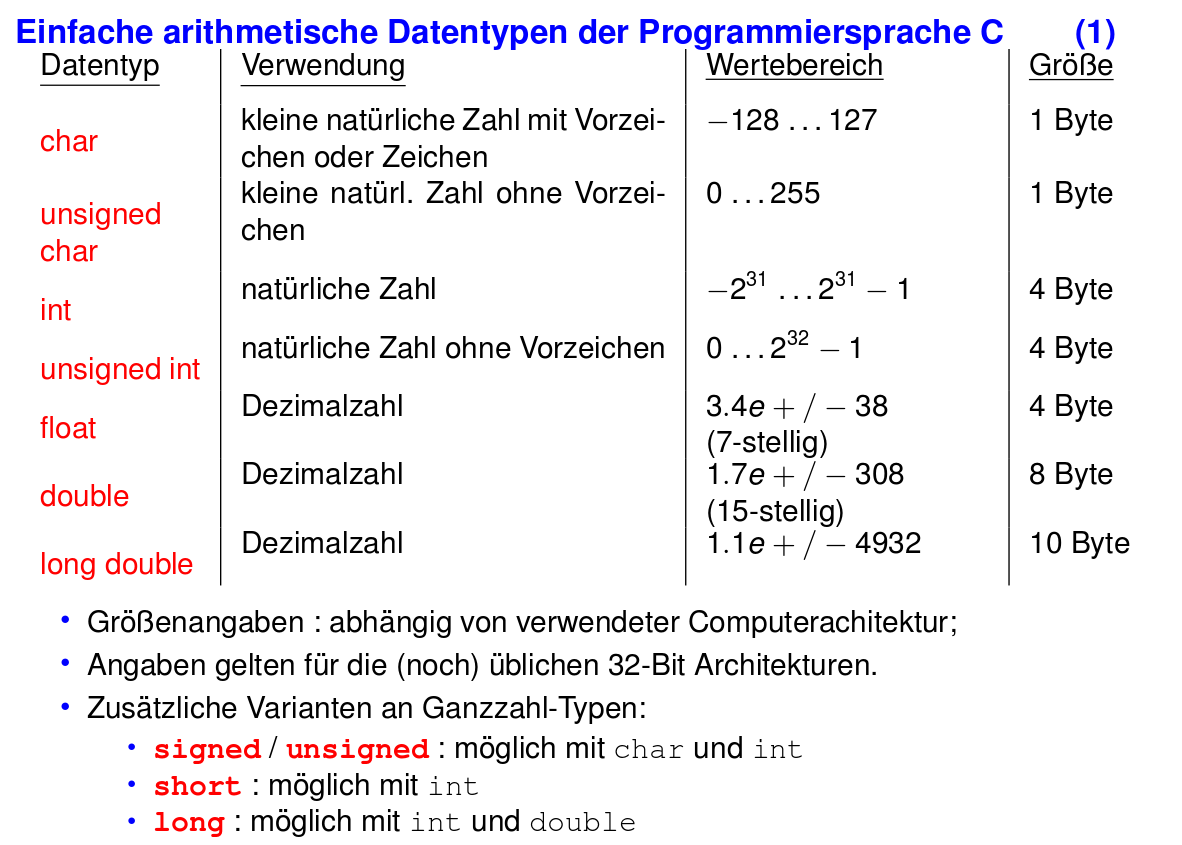
\includegraphics[width=1\textwidth]{ElementareDatentypen.png}
	\caption{Elementare Datentypen in C, Quelle: \cite{2}}
	\label{fig:2}
\end{figure}

%++++++++++++++++++++++++++++++++++++++++++++++++++++++++++++++++++++++++++++
%					  2.2  Variablen Deklaration
%++++++++++++++++++++++++++++++++++++++++++++++++++++++++++++++++++++++++++++
\subsection{Variablen Deklaration}
\label{sec:22}


\begin{lstlisting}
//Variablen Deklaration und Initialisierung
int var1, var2 = 10, var3;

//Konstante festlegen
const int var4 = 21;
\end{lstlisting}

%++++++++++++++++++++++++++++++++++++++++++++++++++++++++++++++++++++++++++++
%					  2.3  Rechenoperationen
%++++++++++++++++++++++++++++++++++++++++++++++++++++++++++++++++++++++++++++
\subsection{Rechenoperationen}
\label{sec:23}


\begin{lstlisting}
int a, b, c;

// Zuweisung eines konstanten Wertes, a ist 1
a = 1;
// Zuweisung eines Variablenwertes, b ist 1
b = a;

// Summe
a = b + c;
// Subtraktion
a = b - c;
// Multiplikation
a = c * b;
// Division
a = c / b;

// a mit Inkrement-Operator hochzaehlen (a = a + 1)
a++;
// a mit Dekrement-Operator erniedrigen (a = a - 1)
a--;

// Erst Zuweisung, dann inkrementieren
a = b++;
// Erst inkrementieren, dann zuweisen
a = ++b;

// Modulo (Restberechnung)
a = b % c;

// Uebernahme des linksseitigen Wertes nach der rechtsseitigen Berechnung (Bsp. a = (b+c)+a)
a += b + c;
a -= b + c;
a *= b + c;
a /= b + c;
a %= b + c;
\end{lstlisting}

%++++++++++++++++++++++++++++++++++++++++++++++++++++++++++++++++++++++++++++
%					  2.4  Logische Operatoren
%++++++++++++++++++++++++++++++++++++++++++++++++++++++++++++++++++++++++++++
\subsection{Logische Operatoren}
\label{sec:24}


\begin{lstlisting}
int a, b, c;

//AND
a = b & c;
//OR
a = b | c;
//XOR
a = b ^ c;
//NOT
a = ~b;

//Bit-shifting
a = b << 1;
c = b >> 1;
\end{lstlisting}

%++++++++++++++++++++++++++++++++++++++++++++++++++++++++++++++++++++++++++++
%					  2.5 Casting (Typumwandlung)
%++++++++++++++++++++++++++++++++++++++++++++++++++++++++++++++++++++++++++++
\subsection{Casting (Typumwandlung)}
\label{sec:25}


\begin{lstlisting}
int a;
float b;

a = (int) b;
\end{lstlisting}

%++++++++++++++++++++++++++++++++++++++++++++++++++++++++++++++++++++++++++++
%					  3.1 Bildschirmausgabe
%++++++++++++++++++++++++++++++++++++++++++++++++++++++++++++++++++++++++++++
\section{Benutzerinteraktion}
\subsection{Bildschirmausgabe}
\label{sec:31}


\noi In den Ausgabestrings können Formatierungsplatzhalter verwendet werden. Damit ist es möglich in einen eigentlich statischen String den Wert einer Variable einzufügen. Als Platzhalter wird der Typ der Variable angegeben und diese anschließend durch Komma getrennt und von links nach rechts gelesen an die Konsolenausgabe mit angehängt. \%c ist der Platzhalter für ein einzelnes Zeichen (Char), \%d für eine ganze Zahl und \%f für eine Gleitkommazahl. Zusätzlich können weitere Formatierungsparamter mit angegeben werden. So kann zum Beispiel mit \qt{\%2.3f} ein Platzhalter definiert werden, der die entsprechende Gleitkommazahl auf zwei Vorkommastellen und 3 Nachkommastellen in der Ausgabe reduziert.

\begin{lstlisting}
float laenge=312.5789, breite=5.6;
printf("\nLaenge: %f cm\nBreite: %f cm\n", laenge, breite);
printf("\nLaenge: %10.2f cm\nBreite: %10.2f cm\n", laenge, breite);
\end{lstlisting}

\begin{lstlisting}[language=bash,  backgroundcolor=\color{pureblack}, basicstyle=\ttfamily\footnotesize\color{purewhite}, rulecolor=\color{slightgray}]
$ Laenge: 312.578888 cm
$ Breite: 5.600000 cm

$ Laenge:     312.58 cm
$ Breite:       5.60 cm
\end{lstlisting}


%++++++++++++++++++++++++++++++++++++++++++++++++++++++++++++++++++++++++++++
%					  3.2 Benutzereingabe
%++++++++++++++++++++++++++++++++++++++++++++++++++++++++++++++++++++++++++++
\subsection{Benutzereingabe}
\label{sec:31}


\noi Einzelnes Zeichen einlesen mit \qt{getchar()}:

\begin{lstlisting}
char c;
printf("Mit welchem Buchstaben beginnt ihr Vorname? ");
c = getchar();
printf("\nIch weiss jetzt, dass Ihr Vorname mit '%c' beginnt.\n", c);
\end{lstlisting}

\noi Platzhalter (\%d und \%f) einlesen mit \qt{scanf()}:

\begin{lstlisting}
int tag, monat, jahr;
printf("Bitte geben Sie ihr Geburtsdatum ein [TT.MM.JJJJ]: ");
scanf("%d.%d.%d", &tag, &monat, &jahr);
printf("\nIhr internationales Geburtsdatum: %04d-%02d-%02d\n", jahr, monat, tag);
\end{lstlisting}

\noi Bei der Benutzereingabe über die Tastatur wird immer die Eingabebestätigung mittels Enter auch von \qt{scanf()} mitgelesen. Daher ist eine temporäre Variable notwendig um die ungewünschte Eingabebestätigung abzufangen.

\begin{lstlisting}
char a, b, temp;

printf("\nGeben sie ein Zeichen ein: ");
scanf("%c%c", &a, &temp);

printf("\nGeben sie ein Zeichen ein: ");
scanf("%c%c", &b, &temp);

printf("\nDie ASCII-Codes ihrer Zeichen sind %d und %d\n", a, b);
\end{lstlisting}


%++++++++++++++++++++++++++++++++++++++++++++++++++++++++++++++++++++++++++++
%					  4.1 Operatoren
%++++++++++++++++++++++++++++++++++++++++++++++++++++++++++++++++++++++++++++
\section{Operatoren und Funktionen}
\subsection{Operatoren}
\label{sec:41}


\noi Vergleichsoperatoren

\begin{lstlisting}
int a = 0,b = 2;

//Gleichheit
if(a == b);

//Ungleich
if(a != b);

//Groesser bzw. groesser gleich
if(a > b);
if(a >= b);

//Kleiner bzw. kleiner gleich
if(a < b);
if(a <= b);
\end{lstlisting}

\noi Logische Operatoren

\begin{lstlisting}
int a = 0,b = 2;

//Negation
if(!a);

//Logisches UND
if(a && b);

//Logisches ODER
if(a || b);
\end{lstlisting}


%++++++++++++++++++++++++++++++++++++++++++++++++++++++++++++++++++++++++++++
%					  4.2 Verzweigungen und Schleifen
%++++++++++++++++++++++++++++++++++++++++++++++++++++++++++++++++++++++++++++
\subsection{Verzweigungen und Schleifen}
\label{sec:42}


\subsubsection{If - Else if - Else}

\begin{lstlisting}
int zahl=6;

if(zahl==5) printf("fuenf\n");
else if(zahl==6) printf("sechs\n");
else printf("nicht fuenf und nicht sechs\n");
\end{lstlisting}

\subsubsection{Switch - Case}

\begin{lstlisting}
int a=2;

switch(a) {
	case 1: printf("a ist eins\n"); break;
	case 2: printf("a ist zwei\n"); break;
	case 3: printf("a ist drei\n"); break;
	default: printf("a ist irgendwas\n"); break;
}
\end{lstlisting}

\subsubsection{While}

\begin{lstlisting}
int i=1;
while(i <= 100) {
	printf("Zahl %d\n", i);
	i++;
}
\end{lstlisting}

\subsubsection{For}

\begin{lstlisting}
int i;

for(i=0; i<5; i++) {
	printf("Zahl %d\n", i+1);
}
\end{lstlisting}

\subsubsection{Do - while}

\begin{lstlisting}
int alter;

do {
    printf("\nBitte geben sie ihr Alter ein: ");
    scanf("%d", &alter);
} while(alter <  5 || alter > 100);

printf("Danke.\n");
\end{lstlisting}

\noi Mit \tbf{break} können alle Schleifen unterbrochen werden, ohne den Kontrollpunkt nochmal zu passieren. Mit \tbf{continue} wird in jeder Schleife direkt zum Kontrollpunkt gesprungen und alle nachfolgenden Argumente somit ignoriert.


%+++++++++++++++++++++++++++++++++++++++++++++++++++++++++++++++++++++++++++++
%					      Literaturverzeichnis
%+++++++++++++++++++++++++++++++++++++++++++++++++++++++++++++++++++++++++++++
\newpage
 %Literaturverzeichnis
\begin{RaggedRight}
\begin{thebibliography}{999}
\addcontentsline{toc}{section}{Literaturverzeichnis}

\bibitem[1]{1} Fischer, Elias: \qt{Das C Tutorial (deutsch)}, \url{http://www.c-howto.de/tutorial-einfuehrung.html}, Abgefragt am: 23.10.2015
\bibitem[2]{2} Spurk, R.: \qt{Datentypen in der Programmiersprache C}, Universität Saarland, 2009, \url{http://www.rw.cdl.uni-saarland.de/teaching/c08/mat/cc++_ws0809.27-10-2008_ElementareDatentypen-Teil1.pdf}, Abgefragt am: 24.10.2015

\end{thebibliography}
\end{RaggedRight}

%+++++++++++++++++++++++++++++++++++++++++++++++++++++++++++++++++++++++++++++
%					      Anhang
%+++++++++++++++++++++++++++++++++++++++++++++++++++++++++++++++++++++++++++++
\newpage
\appendix
\section*{Anhang}
\addcontentsline{toc}{section}{Anhang}

\section{Ascii Tabelle}
\label{sec:A}

\begin{figure}[H]
	\centering
	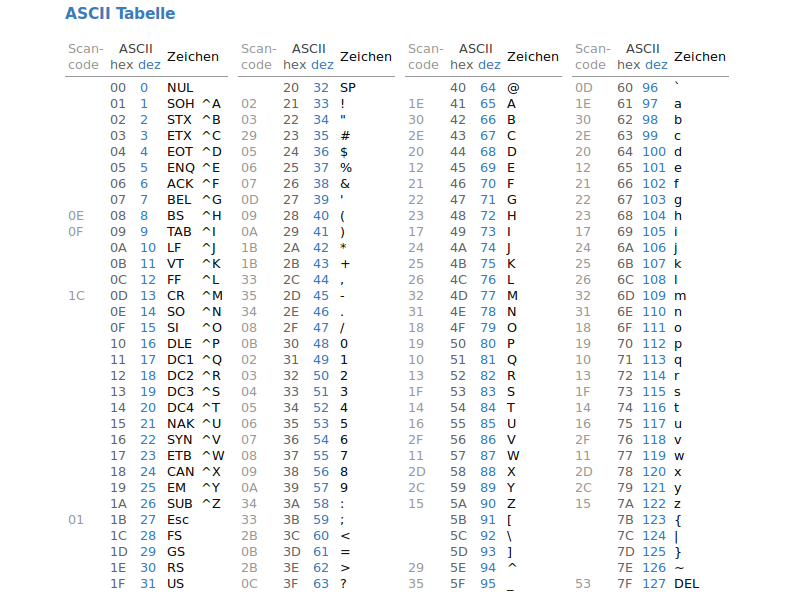
\includegraphics[width=1\textwidth]{ascii.png}
	\caption{Ascii Tabelle, Quelle: \cite{1}}
	\label{fig:1}
\end{figure}

\end{document}
%+++++++++++++++++++++++++++++++++++++++++++++++++++++++++++++++++++++++++++++
%					      ENDE
%+++++++++++++++++++++++++++++++++++++++++++++++++++++++++++++++++++++++++++++


%#######BEISPIELE################
%##Hyperlink##
%\href{URL}{Angezeigter Name}\newline

%##Bild einbinden##
%\begin{figure}[H]
%	\centering
%	\includegraphics[width=0.7\textwidth]{Nr1.png}
%	\caption{Irgendeine Bildbeschreibung, Quelle: Da wo ich es herhabe}
%	\label{fig:1}
%\end{figure}

%##Aufzählung##
%\begin{itemize}
%	\item Hier den Text
%\end{itemize}

%##Quellcode##
%\begin{lstlisting}
%//Testing comments
%for(int i = 0; i < k; i++){
%	ArrayList<Integer> test = new ArrayList<Integer>();
%}
%\end{lstlisting}

%##Tabelle##
%\begin{table}[H]
%	\centering
%	\begin{tabular}{ l | l   }
 %		Inhalt1 & Beschreibung1\\
 %		Inhalt2 & Beschreibung2\\
%		Inhalt3 & Beschreibung3\\
%	\end{tabular}
%\caption{Beispiel Text für eine Tabelle}
%\label{tab:1}
%\end{table}

%##Formel##
%\begin{equation}
% x_{1,2} = \frac{-b \pm \sqrt{ b^2 - 4 a c}}{2a} 
%\label{eq:Gl1}
%\end{equation}

%##Abbildungsverzeichnis#
%\listoffigures

%##Literaturverzeichnis##
%Referenz auf Literaturverzeichnis ueber
%\cite{test}

%\newpage
%\begin{thebibliography}{999}
%\bibitem[1]{test} Kasper, Lars: Die berühmt-berüchtigte Pressekonferenz des Giovanni Trapattoni, \url{http://www.kasper-online.de/docs/trap/}, Stand: 30.10.2013
%\end{thebibliography}

%##Seite Horizontal##
%\begin{landscape}
%\end{landscape}

%Console Commands
%\begin{lstlisting}[language=bash,  backgroundcolor=\color{pureblack}, basicstyle=\ttfamily\footnotesize\color{purewhite}, rulecolor=\color{slightgray}]
%  $ wget http://tex.stackexchange.com
%\end{lstlisting}

%Zahlenkreise
%\kreis{5}
%\ding{192}

%Strukturierter Text
%\begin{lstlisting}[language=C, keywordstyle=\color{blue}, morekeywords={FOR, TO, BY, DO, END_FOR, IF, END_IF, FUNCTION_BLOCK, TRUE, FALSE, THEN, CASE, OF, ADR, SIZEOF, REAL_TO_INT, SQRT, INT_TO_REAL, AND, OR, NOT, ABS, LOG, END_FUNCTION_BLOCK, END_CASE, FUNCTION, END_FUNCTION}]
